\documentclass[a4paper,12pt]{article}

\usepackage{geometry}
\geometry{top=15mm}
\geometry{bottom=30mm}
\geometry{left=10mm}
\geometry{right=20mm}
\linespread{1}
\setlength{\parindent}{12pt}
\setlength{\parskip}{8pt}

\usepackage{titleps}

\newpagestyle{main}
{
  \setheadrule{0.4pt}
  \sethead{}{}{}
  \setfootrule{0,4pt}
  \setfoot{}{\thepage}{}
}
\usepackage{color}
\usepackage[english,russian]{babel}
\usepackage[T2A]{fontenc}
\usepackage[utf8]{inputenc}
\usepackage{amsthm,amsmath,amsfonts,amssymb,mathtools}
\usepackage{indentfirst}
\usepackage{lipsum}
\usepackage{graphicx}
\usepackage{float}
\usepackage{wrapfig}

\newcommand{\partdef}[2]{\frac{\partial \mathnormal{#1}}{\partial \mathnormal{#2}}}

\begin{document}

\begin{center}
\textbf{
Численное решение краевой задачи принципа максимума в задаче оптимального управления методом стрельбы.
}
\end{center}





\section{Постановка задачи.}
Рассматривается задача Лагранжа с фиксированным временным отрезком и без ограничений вида "меньше или равно":
\begin{align}
\begin{align*}
    B_0=\int_0^2\frac{t^r}{1+{\dot x}^2} {dt} \rightarrow {inf} ,\\
    x(0)=0 ,x(2)=1 ,r \in \{1, 2\}\\
    u \in \left[0,16\right] 
\end{align*}
\end{align}

Требуется формализовать задачу, как задачу оптимального управления. Свести задачу принципом максимума Понтрягина к краевой задаче, численно решить полученную задачу методом стрельбы и обосновать точность полученных результатов. Проверить полученные экстремали Понтрягина на оптимальность при различных значениям параметра $r \in \{1, 2\}.$





\section{Формализация задачи.}
Формализуем задачу, как задачу оптимального управления. Для этого обозначим $u= \ddot x, y=\dot x $. Тогда наша задача примет следующий вид:
\begin{align}
\begin{align*}
    \left\{
        \begin{array}{l}
            {\dot x}=y
            \\
            {\dot y}=u
            \\
            u \in \left[0, 16\right]
            \\
            x(0)=0
            \\
            x(2)=1
            \\
            r \in \{1, 2\}
            \\
            B_0=\int_0^2\frac{t^r}{1+{\dot x}^2} {dt} \rightarrow {inf}
        \end{array}
    \right. 
\end{align*}
\end{align}





\section{Система необходимых условий оптимальности.}
Выпишем функции Лагранжа и Понтрягина: 
\begin{align*}
&\mathcal{L}=\int_{0}^{T}\mathbf{L}dt + l,\\
\textrm{ Лагранжиан  } &\mathbf{L}=p_x \cdot (\dot x -y)+p_y \cdot (\dot y -u)+\lambda_0 \cdot \frac{t^r}{1+y^2},\\
\textrm{ Терминант  } &l=\lambda_1 \cdot x(0)+ \lambda_2 \cdot (x(2)-1),\\
&H=p_x \cdot y + p_y \cdot u- \lambda_0 \cdot \frac{t^r}{1+y^2}.
\end{align*}

Применим к задаче оптимального управления (2) принцип максимума Понтрягина. Необхоимые условия оптимальности:

\begin{itemize}
    \item[\text{(a)}]

    Уравнение Эйлера-Лагранжа (сопряженная система уравнений, условие стационарности по 
    $
    \left( 
        \begin{array}{c}
            x \\
            y
        \end{array}
    \right)
    $),
    $
    \left( 
        \begin{array}{c}
            \dot p_x \\
            \dot p_y
        \end{array}
    \right)=-
    \left( 
        \begin{array}{c}
            \partdef{H}{x} \\
            \partdef{H}{y}
        \end{array}
    \right)
    $:
    \begin{align}
    \left\{
    \begin{array}{l}
        \dot p_x = 0\\
        \dot p_y = -p_x - \lambda_0 \frac{2\cdot t^r \cdot y}{{(1+y^2)}^2}
    \end{array}
    \right.
    \end{align}

\item[\text{(б)}]
Условие оптимальности на управление, $u=arg \:abs\: max\: H(u)$:

В нашем случае $H(u)=p_y \cdot u$:
$u=arg \:abs\: max\:(p_y \cdot u )
=
\left\{
\begin{array}{l}
16 \text{ ,если } p_y>0 \\
0 \text{ ,если } p_y<0
\end{array}
\right.
$

\item[\text{(в)}]
Условие трансверсальности по 
$
\left(
\begin{array}{c}
    x \\
    y
\end{array}
\right)
,
p_x(t_k)=(-1)^k \cdot \partdef{l}{x(t_k)},
p_y(t_k)=(-1)^k \cdot \partdef{l}{y(t_k)},
$ где $k\in\{0,1\},t_0=0,t_1=2:$
\begin{align}
    p_y(0)=0,\: p_y(2)=0,\\
    p_x(0)=\lambda_1,\: p_x(2)=-\lambda_2
\end{align}

\item[\text{(г)}]
Условие стационарности по $t_k$:\newline
Нет, так как в задаче (2) $t_k$ - известные константы;

\item[\text{(д)}]
Условие дополняющей нежёсткости:\newline
Нет, так как в задаче (2) отсутсвуют условия вида "меньше или равно"; 

\item[\text{(e)}]
Условие неотрицательности: $\lambda_0 \geq 0.$

\item[\text{(ж)}]
Условие нормировки (множители Лагранжа могут быть выбраны с точностью до положительного множителя);

\item[\text{(з)}]
НЕРОН (множители Лагранжа НЕ Равны Одновременно Нулю).
\end{itemize}





\section{Анормальный случай и исследование задачи.}
Исследуем возможность анормального случая $\lambda_0=0$. Из первого уравнения системы (3) имеем, что $p_x=const=p_x(0).$ Тогда при $\lambda_0=0$ из второго уравнения системы (3) имеем $p_y(t)=p_x(0) \cdot t + p_y(0)$. Но из условия (4) имеем $p_x(0)=0$, что означает, что $\lambda_1=\lambda_2=0$. Тогда получили следующую ситуацию:\newline
в момент времени $t=0$ получили $(\lambda_0,\lambda_1,\lambda_2,p_x,p_y)=O$.
Таким образом если $\lambda_0=0$, то все множители Лагранжа равны 0, что противоречит условию (з).

Так как $\lambda_0 \neq 0$, то можем в силу поункта (ж) положить $\lambda_0=1$, тогда все коэффициенты должны находится однозначно.





\section{Краевая задача.}
Таким образом, на основе принципа Понтрягина задача оптимального управления (2) сводится к краевой задаче. А именно из (2), (3), (4) получаем следующую систему:
\begin{align}
    &\left\{
        \begin{array}{l}
            \dot x =y,\\
            \dot y= u,\\
            \dot p_x= 0\\
            \dot p_y= -p_x -\frac{2\cdot t^r \cdot y}{{(1+y^2)}^2}\\
            u=\left\{
            \begin{array}{l}
                16 \text{ ,если } p_y>0 \\
                0 \text{ ,если } p_y<0
            \end{array}
            \right.
        \end{array}
    \right.
    \\
    &\begin{array}{l}
        x(0)=0, \: x(2)=1,\\
        p_y(0)=0, \: p_y(2)=0,\\
        r \in \{1, 2\}.
    \end{array}
\end{align}





\section{Численное решение краевой задачи методом стрельбы.}
Краевая задача (6)-(7) решается численно методом стрельбы. В качестве параметров пристрелки выбирают недостающие для задачи Коши значения при $t=0$. В нашем случае параметрами пристрелки будут $y(0)=\alpha_1,\:p_x(0)=\alpha_2$. Задав эту пару парметров, мы можем решить задачу Коши на конечном отрезке $\left[0,2\right]$ и получить по соответсвующему выбронному $\overrightarrow{\alpha}=\{\alpha_1,\alpha_2\} $ функции 
$
x(\cdot)\left[\alpha_1,\alpha_2\right],\:
y(\cdot)\left[\alpha_1,\alpha_2\right],\:
p_x(\cdot)\left[\alpha_1,\alpha_2\right],\:
p_y(\cdot)\left[\alpha_1,\alpha_2\right]
$. В частности можем получить 
$
y(2)\left[\alpha_1,\alpha_2\right],\:
p_x(2)\left[\alpha_1,\alpha_2\right]
$.
Задача Коши для системы дифференциальных уравнений (6) с начальными условиями (7), заданнымии в момент времени $t=0$, с учетом заданного $\overrightarrow{\alpha}$ решается численно явным способом, а имеено с помощью метода Рунге-Кутты 8-го порядка, основанным на расчетных формулах Дормана-Принса 8(7) DOPRI8 с автоматическим выбором шага(то есть с контролем относительной локальной погрешности на шаге по правилу Рунге). Для решения нашей краевой задачи нужно подобрать $\overrightarrow{\alpha}$ таким образом, чтобы выполнились условия:

\begin{align}
\begin{align*}
x(2)\left[\alpha_1,\alpha_2\right]-1=0,\\
p_y(2)\left[\alpha_1,\alpha_2\right]=0
\end{align*}
\end{align}

Тогда можем определить вектор функцию невязок 
$
X(\overrightarrow{\alpha})=
\begin{pmatrix}
    x(2)\left[\alpha_1,\alpha_2\right]-1\\
    p_y(2)\left[\alpha_1,\alpha_2\right]
\end{pmatrix}$.
Таким образом, выбирая для решения краевой задачи метод стрельбы, решение краевой задачи свелось к решению двух алгебраических уравнений от двух неизвесных, а именно 
$
X(\overrightarrow{\alpha})=0
$.
Корень $\overrightarrow{\alpha}$ системы алгебраических уравнений $X(\overrightarrow{\alpha})=0$ находится методом Ньютона с модификацией Исаева-Сонина. Решение линейной системы уравнений внутри модифицированного метода Ньютона осуществляется методом Гаусса с выбором главного элемента по столбцу, с повторным пересчетом.
В нашей задаче крайне важен следующий тест части программы, решающей задачу Коши, на системе дифференциальных уравнений с известным аналитическим решением.





\section{Тест  решения задачи Коши - гармонический осциллятор}

В таблице ниже приведены результаты численного интегрирования системы дифференциальных уравнений гармонического осциллятора $
\left\{
\begin{array}{l}
    \dot x\;=\; y\\
    \dot y\;=\; -x\\
\end{array}
\right.
$  с начальными условиями  $
\left\{
\begin{array}{l}
    x(0)=0\\
    y(0)=1\\
\end{array}
\right.
$ явным методом Рунге-Кутты с оценкой погрешности на шаге через 8-ую производную для различного конечного времени $T$ и различных значений максимально допустимой относительной погрешности на шаге интегрирования $\Delta_{loc}$ . $Steps$ - общее число сделанных шагов интегрирования (число принятых шагов); $|x(T)|$ и $|y(T)-\mathds{cos}(T)|$ - невязки в конце;  $\Delta x(\cdot)$ и $\Delta y(\cdot)$ - максимальное отличие полученного решения от известного аналитического $
\left\{
\begin{array}{l}
    x(t)=\mathnormal{sin}(t)\\
    y(t)=\mathds{cos}(t)
\end{array}
\right.
$  по всем шагам;  $\delta_K(T)$ - оценка глобальной погрешности по формуле $\delta_K(t_{i+1})=r_i+\delta_K(t_i)\cdot e^{L_i}$ , где $r_i$ -  главный член в оценке локальной погрешности, а $L_i=\int_{t_i}^{t_{i+1}} \mu dt; \;\mu $ - логарифмическая норма матрицы Якоби исходной системы дифференциальных уравнений, $
J=
\left(
\begin{tabular}{cc}
    0&1\\
    -1&0\\
\end{tabular}
\right)
$ , равная максимальному собственному  значению матрицы $\frac{(J+J^T)}{2}=
\left(
\begin{tabular}{cc}
    0&0\\
    0&0\\
\end{tabular}
\right)
$ , то есть 0 $\Rightarrow \delta_K(t_{i+1})= r_{i+1} +\delta_K(t_i)\; ;
R_x = \left|\frac{x_{10^{-8}}(T)-x_{10^{-10}}(T)}{x_{10^{-10}}(T)-x_{10^{-12}}(T)}\right| \; , \; R_y= \left|\frac{y_{10^{-8}}(T)-y_{10^{-10}}(T)}{y_{10^{-10}}(T)-y_{10^{-12}}(T)}\right|$ .
 
В таблице ниже представлены полученные данные:

\begin{table}[H]
\begin{tabular}{|c|c|c|c|c|c|c|c|c|c|}
    \hline
    $T$&$\Delta_{loc}$&$Steps$&$|x(T)|$&$|y(T)-\cos(T)|$&$\Delta x(\cdot)$&$\Delta y(\cdot)$&$\delta_K(T)$&$R_x$&$R_y$\\
    \cline{1-10}
    &$ 10^{-08} $&$  6  $&$ 1.99\cdot 10^{-08} $&$ 1.26\cdot 10^{-08} $&$ 1.45\cdot 10^{-08} $&$ 1.42\cdot 10^{-08} $&$ 2.04\cdot 10^{-08} $&$ $& \\
    \cline{2-8}
    $\pi $&$ 10^{-10} $&$ 10 $&$ 2.24\cdot 10^{-10} $&$ 3.42\cdot 10^{-10} $&$ 2.57\cdot 10^{-10} $&$ 2.57\cdot 10^{-10} $&$ 3.61\cdot 10^{-10} $&$ 88.73 $&$ 36.41 $\\
    \cline{2-8}
    &$ 10^{-12} $&$ 17 $&$ 2.29\cdot 10^{-12} $&$ 6.71\cdot 10^{-12} $&$ 4.55\cdot 10^{-12} $&$ 4.48\cdot 10^{-12} $&$ 6.29\cdot 10^{-12} $&$ $& \\
    \cline{1-10}
    &$ 10^{-08} $&$ 53 $&$ 2.00\cdot 10^{-07} $&$ 1.27\cdot 10^{-07} $&$ 1.44\cdot 10^{-07} $&$ 1.44\cdot 10^{-07} $&$ 2.05\cdot 10^{-07} $&$ $&\\
    \cline{2-8}
    $10\cdot \pi $&$ 10^{-10} $&$ 93 $&$ 2.23\cdot 10^{-09} $&$ 3.41\cdot 10^{-09} $&$ 2.56\cdot 10^{-09} $&$ 2.56\cdot 10^{-09} $&$ 3.60\cdot 10^{-09} $&$89.82$&$37.03$\\
    \cline{2-8}
    &$ 10^{-12} $&$ 165 $&$ 2.31\cdot 10^{-11} $&$ 6.79\cdot 10^{-11} $&$ 4.57\cdot 10^{-11} $&$ 4.57\cdot 10^{-11} $&$ 6.39\cdot 10^{-11} $&$ $&\\
    \cline{1-10}
    &$10^{-08}$&$ 522$&$ 2.00\cdot 10^{-06}$&$  1.27\cdot 10^{-06}$&$  1.44\cdot 10^{-06}$&$  1.44\cdot 10^{-06}$&$  2.05\cdot 10^{-06}$&&\\
    \cline{2-8}
    $10^2 \cdot \pi$&$10^{-10}$&$ 926$&$ 2.24\cdot 10^{-08}$&$  3.43\cdot 10^{-08}$&$  2.57\cdot 10^{-08}$&$  2.57\cdot 10^{-08}$&$  3.62\cdot 10^{-08}$&$89.41$&$36.87$\\ 
    \cline{2-8}
    &$10^{-12}$&$ 1645$&$ 2.31\cdot 10^{-10}$&$  6.80\cdot 10^{-10}$&$  4.58\cdot 10^{-10}$&$  4.58\cdot 10^{-10}$&$  6.40\cdot 10^{-10}$&&\\
    \cline{1-10}
    &$10^{-08}$&$ 5216$&$  2.00\cdot 10^{-05}$&$  1.27\cdot 10^{-05}$&$  1.44\cdot 10^{-05}$&$  1.44\cdot 10^{-05}$&$  2.05\cdot 10^{-05}$& &\\
    \cline{2-8}
    $10^3 \cdot \pi$&$10^{-10}$&$ 9252$&$  2.24\cdot 10^{-07}$&$  3.43\cdot 10^{-07}$&$  2.57\cdot 10^{-07}$&$  2.57\cdot 10^{-07}$&$  3.62\cdot 10^{-07}$&$89.49$&$36.90$\\ 
    \cline{2-8}
    &$10^{-12}$&$ 16441$&$  2.31\cdot 10^{-09}$&$  6.80\cdot 10^{-09}$&$  4.58\cdot 10^{-09}$&$  4.58\cdot 10^{-09}$&$  6.40\cdot 10^{-09}$& &\\
    \cline{1-10}
    &$10^{-08}$&$ 52155$&$  2.00\cdot 10^{-04}$&$  1.27\cdot 10^{-04}$&$  1.44\cdot 10^{-04}$&$  1.44\cdot 10^{-04}$&$  2.05\cdot 10^{-04}$& &\\
    \cline{2-8}
    $10^4 \cdot \pi$&$10^{-10}$&$ 92519$&$  2.24\cdot 10^{-06}$&$  3.43\cdot 10^{-06}$&$  2.57\cdot 10^{-06}$&$  2.57\cdot 10^{-06}$&$  3.62\cdot 10^{-06}$&$89.48$&$36.90$\\
    \cline{2-8}
    &$10^{-12}$&$ 164407$&$  2.25\cdot 10^{-08}$&$  6.80\cdot 10^{-08}$&$  4.58\cdot 10^{-08}$&$  4.58\cdot 10^{-08}$&$  6.40\cdot 10^{-08}$& &\\
    \cline{1-10}
    &$10^{-08}$&$ 521580$&$  2.00\cdot 10^{-03}$&$  1.27\cdot 10^{-03}$&$  1.44\cdot 10^{-03}$&$  1.44\cdot 10^{-03}$&$  2.05\cdot 10^{-03}$& &\\
    \cline{2-8}
    $10^5 \cdot \pi$&$10^{-10}$&$ 925185$&$  2.24\cdot 10^{-05}$&$  3.43\cdot 10^{-05}$&$  2.57\cdot 10^{-05}$&$  2.57\cdot 10^{-05}$&$  3.62\cdot 10^{-05}$&$89.60$&$36.85$\\
    \cline{2-8}
    &$10^{-12}$&$ 1644068$&$  2.45\cdot 10^{-07}$&$  6.80\cdot 10^{-07}$&$  4.58\cdot 10^{-07}$&$  4.58\cdot 10^{-07}$&$  6.40\cdot 10^{-07}$& &\\
    \cline{1-10}
    &$10^{-08}$&$ 5219496$&$  2.02\cdot 10^{-02}$&$  1.26\cdot 10^{-02}$&$  1.44\cdot 10^{-02}$&$  1.44\cdot 10^{-02}$&$  2.05\cdot 10^{-02}$& &\\
    \cline{2-8}
    $10^6 \cdot \pi$&$10^{-10}$&$ 9252025$&$  2.24\cdot 10^{-04}$&$  3.43\cdot 10^{-04}$&$  2.57\cdot 10^{-04}$&$  2.57\cdot 10^{-04}$&$  3.62\cdot 10^{-04}$&$89.99$&$36.38$\\
    \cline{2-8}
    &$10^{-12}$&$ 16440684$&$  2.22\cdot 10^{-06}$&$  6.80\cdot 10^{-06}$&$  4.58\cdot 10^{-06}$&$  4.58\cdot 10^{-06}$&$  6.40\cdot 10^{-06}$& &\\
    \cline{1-10}
\end{tabular}
\end{table}

\newpage




\section{Аналитическое решение задачи.}

Отыскание общего решения данной системы является достаточно тяжелой задачей, поэтому наша цель будет найти такие решения, которые удовлетворяютя данной системе. Итак, имеем следующую систему уравнеий:

\begin{align*}
    &\left\{
        \begin{array}{l}
            \dot x =y,\\
            \dot y= u,\\
            \dot p_x= 0\\
            \dot p_y= -p_x -\frac{2\cdot t^r \cdot y}{{(1+y^2)}^2}\\
            u=\left\{
            \begin{array}{l}
                16 \text{ ,если } p_y>0 \\
                0 \text{ ,если } p_y<0
            \end{array}
            \right.
        \end{array}
    \right.
    \\
    &\begin{array}{l}
        x(0)=0, \: x(2)=1,\\
        p_y(0)=0, \: p_y(2)=0,\\
        r \in \{1, 2\}.
    \end{array}
\end{align*}

Задаем начальные условия:
\begin{align}
    x(0)=0\:\:,\:\:y(0)=y_0\:\:,\:\:p_y(0)=0\:\:,\:\:p_x(0)=p_x^0.
\end{align}

Решим для начала задачу с параметром $r=1.$

\textbf{Будем считать, что $p_x^0 > 0.$} Тогда имеем $\dot p_y(0)<0$, что означает, что необходимо выставить параметр $u=0.$. Решая эту систему уравнеий получаем следующие решения:

\begin{align*}
    \left\{
        \begin{array}{l}
            x(t)\;=\; y_0\cdot t\\
            y(t)\; \equiv \; y_0\\
            p_x(t)\;\equiv \; p_x^0\\
            p_y(t)\; =\; -p_x^0\cdot t\;-\;\frac{y_0}{(1+y_0^2)^2\cdot t^2}
        \end{array}
    \right.
\end{align*}

Пусть $t^*$ - момент, когда $p_x(t^*)\;=\;0\;.$ Заметим лишь, что если $y_0\;=\; 0$ , то имеем противоречие  с $p_y(2)=0$.
Тогда для этого момента времени справедливо:

\begin{align*}
    \left\{
        \begin{array}{l}
            x(t^*)\;=\;   y_0\cdot t^*\\
            y(t^*)\;=\;   y_0\\
            p_x(t^*)\;=\; p_x^0\\
            p_y(t^*)\;=\; 0
        \end{array}
    \right.
    \;\;\; \text{,где  } t^* \;=\; \frac{p_x^0 \cdot (1+y_0^2)^2}{- y_0 } . 
\end{align*}

\begin{align*}
&t^* \;>\; 0 \Rightarrow y_0\;<\;0\;\\
&t^* \in \left(0\:,\:2\rigth] \text{ , причем если } t^* \;=\; 2 \text{ , то имеем противоречие с } x(2)=1; \;\Rightarrow\; \\
& \;\Rightarrow\; t^* \in \left(0\:,\:2\right) \Leftrightarrow  \;0\;<\; p_x^0\; < \; \frac{-2 \cdot y_0}{(1+y_0^2)^2}
\end{align*}

Заметим, что $\dot p_y(t^*)=p_x^0 \;>\;0 $ , что означает, что решение переходит в верхнюю полуплоскость трансверсально, поэтому после точки $t^*$ считаем $u=16$ . Для удобства совершим сдвиг по оси времени $t\;=\;\tau + t^*$, и тогда  новая систеа примет следующий вид:

\begin{align*}
    \left\{
        \begin{array}{l}
            \dot x\;=\; y,\\
            \dot y\;=\; u,\\
            \dot p_x\;=\; 0\\
            \dot p_y\;=\; -p_x -\frac{2\cdot (\tau + t^*) \cdot y}{{(1+y^2)}^2}\\
        \end{array}
    \right.
\;\;\; \text{, с начальными условиями }
    \left\{
        \begin{array}{l}
            x(0)\;=\;   y_0\cdot t^*\\
            y(0)\;=\;   y_0\\
            p_x(0)\;=\; p_x^0\\
            p_y(0)\;=\; 0
        \end{array}
    \right.
\end{align*}

Решаем эту систему уравнений и получаем следующее решение:
\begin{align*}
    \left\{
        \begin{array}{l}
            x(\tau)\;=\; 8 {\tau}^{2}+\tau \cdot y_0 + y_0 \cdot t^*\\
            y(\tau)\;=\; 16 \tau + y_0\\
            p_x(\tau)\;=\; p_x^0\\
            p_y(\tau)\;=\; \frac{1}{256}\left(
                16 \left(
                    -16\cdot p_x^0 \cdot \tau - \frac{t^*}{1+y_0^2} + \frac{\tau + t^*}{1+(16 \cdot \tau + y_0)^2}
                \right)+
                \mathbf{Arctan}(y_0)-
                \mathbf{Arctan}(16 \tau + y_0)
            \right)
        \end{array}
    \right.
\end{align*}

Попытаемся найти такие начальные значения, что будут выполнены краевые условия, то есть:

\begin{align*}
    \left\{
        \begin{array}{l}
            x(2-t^*)\;=\;1 \\
            p_y(2-t^*)\;=\;0
        \end{array}
    \right.
    \;\;\;\text{ , причем } p_x^0 \;=\; -\frac{t^* \cdot y_0}{(1+y_0^2)^2}
    \\
    x(2-t^*)\;=\;1\; \Rightarrow \; t^*\;=\;2\;\pm \frac{\sqrt{2}}{4}\sqrt{1-2\cdot y_0}\text{ , }
    \\
    \text{ также необходимо вспомнить об ограничении }t^*\in\left(0,2\right)\text{ ,}
    \\
    \left[
    \begin{array}{l}
        t^*\;=\;2\;+ \frac{\sqrt{2}}{4}\sqrt{1-2\cdot y_0}\;>2\;\text{ для }\forall y_0\;<\;0\text{ -противоречие.}
        \\
        t^*\;=\;2\;- \frac{\sqrt{2}}{4}\sqrt{1-2\cdot y_0}\;\Rightarrow\; -\frac{31}{2}\;<\;y_0\;<\;0
    \end{array}
    \right.
    \\
    \text{подставляя соответствующие функции в последнее уравннение системы }\Rightarrow 
\end{align*}

\begin{multline*}
    \frac{4(-8+\sqrt{2-4\cdot y_0})}{1+y_0^2}+{}\\
    {}+32 \cdot \frac{\sqrt{2-4\cdot y_0}(132\cdot y_0-264\cdot y_0^2+20\cdot y_0^3)+(1-33\cdot y_0+196\cdot y_0^2-257\cdot y_0^3+3\cdot y_0^4)}{(1+y_0^2)^2\cdot (33+8(-8+\sqrt{2-4 \cdot y_0})\cdot y_0 +y_0^2)}+{}\\
    {}+\mathbf{Arctan}(y_0)-
    \mathbf{Arctan}(4\sqrt{2-4\cdot y_0}+ y_0)\;=\; 0
\end{multline*}

\begin{wrapfigure}{r}{0.4\textwidth}
    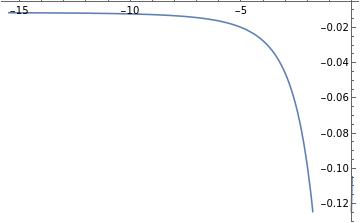
\includegraphics[width=0.4\textwidth]{img1.png}
\end{wrapfigure}

Из рисунка видно, что последнее уравнение не разрешимо на промежутке $-\frac{31}{2}\;<\;y_0\;<\;0$ .
Причем из рисунка также видно, что $p_y(2-t^*)$ в зависимости от $y_0$ может принимать как положительные, так и отрицатеьные значения, поэтому опять найдется точка переключения со своими ограничениями. После точки переключения управление $u\;=\;0$ .

Это породит новую систему уравнений со своими начальными условиями, с учетом сдвигом по времени эту систему можно записать так:

Для удобства введем обозначения $t_1\:=\: t^*$ , $t_2$ -момент времени, когда посленяя функция $p_y(t2)\;=\;0$ . 

\begin{align*}
    \left\{
        \begin{array}{l}
            \dot x\;=\; y \\
            \dot y \;=\;0 \\
            \dot p_x \;=\;0\\
            \dot p_y \;=\; -p_x - \frac{2\cdot (t+t_1+t_2)\cdot y}{(1+y^2)^2}
        \end{array}
    \right.
    \text{  ,}
\end{align*}
с начальными условиями 
\begin{align*}
    \left\{
        \begin{array}{l}
            x(0)\;=\; x_2 \\
            y(0) \;=\; y_2 \\
            p_x(0) \;=\; p_x^0\\
            p_y(0) \;=\; 0
        \end{array}
    \right.
    \;\;\; \text{ , где }
    \left\{
        \begin{array}{l}
            x_2\;=\; 8 t_2^2 + t_2\cdot y_0 + y_0 \cdot t_1 \\
            y_2 \;=\; 16 t_2 + y_0 \\
            t_1 \;=\; \frac{p_x^0 \cdot (1+y_0^2)^2}{- y_0 }
        \end{array}
    \right.
\end{align*}
Далее хотим разрешить краевую задачу.  Решение системы уравнений примет вид:
\begin{align*}
    \left\{
        \begin{array}{l}
            x(t)\;=\; x_2\cdot t +x_2 \\
            y(t) \;=\; y_2 \\
            p_x(t) \;=\; p_x^0\\
            p_y(t) \;=\; t\left( -p_x^0 - \frac{2\cdot (t_1 + t_2)\cdot y_2}{(1+y_2^2)^2}-\frac{t^\cdot y_2}{(1+y_2^2)^2} \right)=t\cdot \psi(t,t_2,t_1,y_2,p_x^0)
        \end{array}
    \right.
\end{align*}

Опишем идею построения уравнений :

\begin{align*}
\left.
\begin{array}{l}
    \left.
    \begin{array}{l}
        t_1\:=\:t_1(y_0,p_x^0) \Rightarrow p_x^0\:=\:p_x^0(y_0,t_1)
        \\
        \left.
        \begin{array}{l}
                y_2 \:=\: y_2(y_0,t_2)\\
                x_2 \:=\: x_2(t_2,t_1,y_0)\\
                x(2-t_1-t_2)\:=\: \phi(y_2,x_2,t_1,t_2) \:=\:1
        \end{array}
        \right\} \Rightarrow t_1 \:=\: t_1(t_2,y_0)
    \end{array}
    \right\} \Rightarrow p_x^0\:=\:p_x^0(y_0,t_2)
    \\
    \psi(2-t_1-t_2,t_2,t_1,y_2,p_x^0)\:=\:0
\end{array}
\right\} \Rightarrow f(t_2,y_0)\:=\:0 .
\end{align*}

\begin{wrapfigure}[10]{l}[26pt]{0.4\textwidth}
    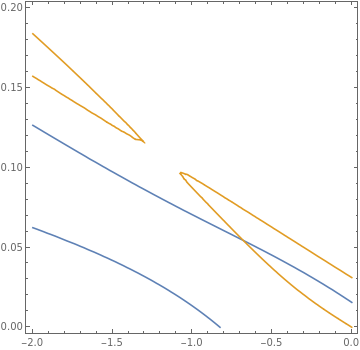
\includegraphics[width=0.4\textwidth]{img2.png}
    \caption{
        \begin{array}{r}
            y_0=-0.681078049\\
            t_2=0.054491750283
        \end{array}
        }
\end{wrapfigure}


А также вспоминая предшествующее уравнение $p_y(t_2)=0 \Leftrightarrow G(t_2,t_1,y_0,p_x^0)\:=\:0$ и совершая аналогичный ряд действия, имеем:

\begin{align*}
    \begin{array}{l}
            f(t_2,y_0)\:=\:0
            \\
            g(t_2,y_0)\:=\:0
    \end{array}
\end{align*}

Было найда пара точек (рис.1 и рис.2), которые могут претедовать на решение, но не одна из точек не подхоит, так как вычесленное по ним время $t_1 \:<\:0$ .

\newpage


\begin{wrapfigure}[15]{l}[26pt]{0.4\textwidth}
        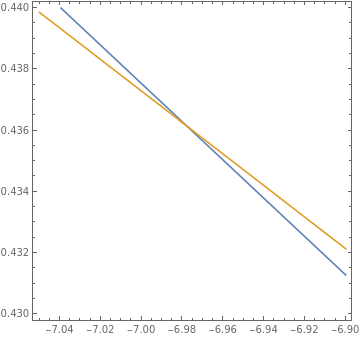
\includegraphics[width=0.4\textwidth]{img3.png}
        \caption{
            \begin{array}{r}
                y_0=-6.977892188\\
                t_2=0.43614901116
            \end{array}
            }
\end{wrapfigure}
Таким образом мы можем далее искать точку переключения и продолжать решение, но это уже сложная задача, поэтому будем пытаться найти решение среди других начальных параметров.

\textbf{Далее будем считать, что $p_x^0=0$ .} 
Заметим, что $y(0)=y_0 \neq 0$, так как решения, тождественно равные 0 нас не интересуют. Таким образом задача распадается на два случая:

Пусть $y_0 > 0$ . Тогда для достаточно маленьково $\delta$ верным будет утверждение, что $\dot p_y(\tau) < 0$ на всем промежутке $\left(0,\delta \right)$. Так как $p_y(0)=0$ , то необходимо брать $u=0$. Это приведет к тому, что:
\begin{align*}
    p_y(t)=&\frac{- t^2\cdot y_0}{(1+y_0^2)^2} \Rightarrow \\ & \nexists \text t_1\text{ , что }p_y(t_1)=0\text{ , что приводит к противоречию.}
\end{align*}
Пусть $y_0 < 0$ . Тогда для достаточно маленьково $\delta$ верным будет утверждение, что $\dot p_y(\tau) > 0$ на всем промежутке $\left(0,\delta \right)$. Так как $p_y(0)=0$ , то необходимо брать $u=16$. Это приведет к тому, что:

\begin{align*}
    p_y(t)=\frac{\mathbf{Arctan}(y_0)-\mathbf{Arctan}(16\cdot t+y_0)}{256}+\frac{t}{16(1+(16\cdot t+y_0)^2)}
    \\
    \begin{array}{c}
        x(t)=8 t^2+t\cdot y_0 \text{ , требуем, чтобы }p_y(2)=0 \text{ и }x(2)=1 .
        \\
        x(2)=1 \; \Rightarrow \; y_0=-\frac{31}{2} \; \Rightarrow \; p_y(2) \neq 0.
    \end{array}
\end{align*}

Это означает, что следует искать точку переключения $t_1$ , затем строить новую систему уравнений и ее решать, в ходе чего будет получено:
Для удобства считаем, что произошел сдвиг по времени.
\begin{align*}
    p_y(t)=\frac{- t^2\cdot y_1}{(1+y_1^2)^2}\text{ , где }y_1=16*t_1+y_0.
\end{align*}
Таким образом имеем, что необходимо выполение $y_1=0$ , иначе невозможно выполнение краевых условие. Тогда имеем уравнение $t_1=t_1(y_0)$ , подстановка которого в $p_y(t_1)=0$ ,полученного на первом шаге дает противоречие, значит решение вообще невозможно при $p_x^0=0$.

\textbf{ Тогда разберемся с последним случаем $p_x^0<0$ .}

\begin{wrapfigure}[11]{r}[26pt]{0.4\textwidth}
    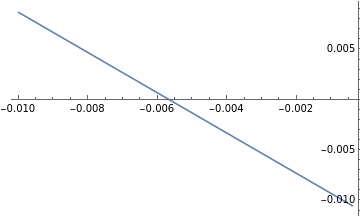
\includegraphics[width=0.4\textwidth]{img4.png}
    \caption{$p_x^0=-0.00566313$}
\end{wrapfigure}

Тогда $\dot p_y(0)>0$ , и в качестве параметра необходимо взять $u=16$ . Тогда получим систему, решением которого имеет вид:

\begin{align*}
    \left\{
        \begin{array}{l}
            x(t)=8 t^2\cdot y_0\\
            y(t)=16 t+y_0\\
            p_x(t) \equiv p_x^0\\
            p_y(t)=-p_x^0\cdot t+\frac{\mathbf{Arctan}(y_0)-\mathbf{Arctan}(16\cdot t+y_0)}{256}+\frac{t}{16(1+(16\cdot t+y_0)^2)}
        \end{array}
    \right.
\end{align*}
Тогда попытаемся решыть такую систему:
\begin{align*}
    \begin{array}{l}
        x(2)=1\;\Rightarrow \; y_0=-\frac{31}{2}\\
        p_y(2)=0\text{ , при} y_0=-\frac{31}{2} \; \Rightarrow \; p_x^0=-0.00566313
    \end{array}
\end{align*}

Таким образом мы нашли решение, не имеющее точки переключения с начальными параметрами $(p_x^0,y_0)=(-0.00566313,-\frac{31}{2})$.
\newline
\begin{wrapfigure}[15]{l}[26pt]{0.4\textwidth}
    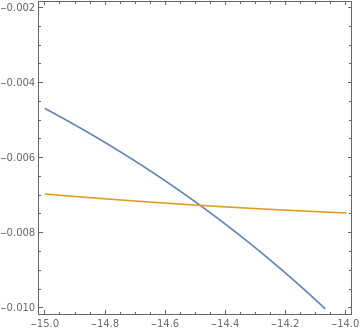
\includegraphics[width=0.4\textwidth]{img5.png}
    \caption{
        \begin{array}{l}
            $p_x^0=-0.00725785633$\\
            $y_0=-14.4849204322$
        \end{array}
        }
\end{wrapfigure}

Попытаемся теперь построить решение, проходящее через одну точку переключения.
Тогда получим новую систему уравнений(с учетом сдвига по времени и сменой значения параметра на 0):


\begin{align*}
    \left\{
        \begin{array}{l}
            \dot x \equiv y_1\\
            \dot y \equiv 0\\
            p_x(t) \equiv p_x^0\\
            \dot p_y=-p_x^0-\frac{2(t+t_1)\cdot y_1}{(1+y_1^2)^2}
        \end{array}
    \right.
    \text{ , где }
    \left\{
        \begin{array}{l}
            x(0) \;=\; x_1 \;=\; 8t_1^2+t_1\cdot y_0\\
            y(0) \;=\; y_1 \;=\; 16t_1+y_0\\
            p_y(0)=0
        \end{array}
    \right.
    \;\;\Rightarrow
    \\
    \\
    \left\{
        \begin{array}{l}
            x(t) \;=\; y_1\cdot t+ x_1\\
            y(t) \;=\; y_1 \\
            p_y(t)=- p_x^0\cdot t-\frac{t^2\cdot y_1}{(1+y_1^2)^2}-\frac{2t\cdot t_1\cdot y_1}{(1+y_1^2)^2}
        \end{array}
    \right.
    \text{ , где }
\end{align*}
\newline
\begin{align*}
    0=-p_x^0\cdot t_1&+\frac{\mathbf{Arctan}(y_0)-\mathbf{Arctan}(16\cdot t_1+y_0)}{256}
    \\
    +&\frac{t_1}{16(1+(16\cdot t_1+y_0)^2)} \Leftrightarrow f_2(y_0,t_1,p_x^0)=0
\end{align*}
\begin{aling*}
    \\
    x(2-t1) \;=\; y_1\cdot (2-t1)+ x_1 \;=\;1 \Rightarrow t_1=\frac{1}{2}(4-\sqrt{16+y_0})
    \\
    \\
    \begin{array}{l}
        \left\{
            \begin{array}{l}
                p_y(2-t_1)=0\\
                t_1=t_1(y_0)\\
                y_1=y_1(y_0,t_1)
            \end{array}
        \right.
        \;\Rightarrow\; F_1(p_x^0,y_0)=0
        \\
        \\
        \left\{
            \begin{array}{l}
                f_2(y_0,t_1,p_x^0)=0\\
                t_1=t_1(y_0)
            \end{array}
        \right.
        \;\Rightarrow\; F_2(p_x^0,y_0)=0
    \end{array}
    \;\Rightarrow\; 
    \left\{
        \begin{array}{l}
            F_2(p_x^0,y_0)=0\\
            F_1(p_x^0,y_0)=0
        \end{array}
    \right.
\end{align*}

Решая эту систему, находим точку $(p_x^0,y_0)=(-0.00725785633,-14.4849204322)$ осталось проверить, что эта точка определяет допустимое $t_1$ .

\begin{align*}
    t_1=\frac{1}{2}(4-\sqrt{16+y_0}) \;\Rightarrow\; t_1=1.384553 \in \left(0,2\right) \;\Rightarrow\;\text{удовлетворяет ограничениям на время.}
\end{align*}

\begin{wrapfigure}[11]{r}[26pt]{0.4\textwidth}
    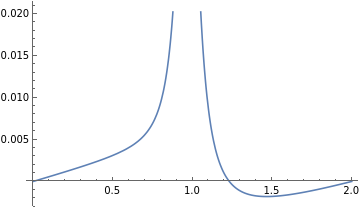
\includegraphics[width=0.3\textwidth]{img6.png}
\end{wrapfigure}

\begin{array}{l}
    $(p_x^0,y_0)=(-0.00566313,-\frac{31}{2})$
    \\
    \text{ - без точек переключения .}
    \\
    $(p_x^0,y_0)=(-0.00725785633,-14.4849204322)$
    \\
    \text{ - с одной точкой переключения.}
\end{array}

Но если для первой пары точек явно постоить функцию $p_x^0$ , то увидем, что у этой функции на самом деле должна быть точка переключения, чего мы не обнаружили.

\begin{wrapfigure}[11]{r}[26pt]{0.4\textwidth}
    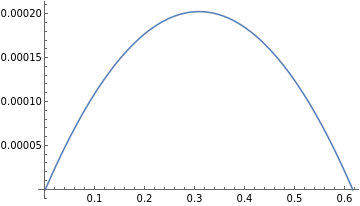
\includegraphics[width=0.3\textwidth]{img7.png}
\end{wrapfigure}
А если посмотреть на вторую пару точек и явно построим $p_x^0$ после первой точки переключения, то увидем, что график расположен выше оси, что противоречит выбору управления.

Поэтому оба нами найденных "решения" таковыми не являются.





\end{document}